\title{LEZIONE 13 31/03/2020}\newline
\textbf{link} \href{https://web.microsoftstream.com/video/22a546ac-3e6b-43e0-b0f9-45a630661700?list=user&userId=faa91214-a6f5-40d7-8875-253fd49b8ce1}{clicca qui}
\begin{itemize}
    \item $G_b(s)= \frac{1}{s^g} \rightarrow G(j \omega) = \frac{1}{(j \omega)^g} \rightarrow \begin{cases}
        |G_b(j \omega)| = \frac{1}{\omega^g} \rightarrow |G_b(j \omega)|_{dB}= - 20 g log(\omega)\\
        arg(G_b(j \omega)) = - g \cdot 90^o
    \end{cases} $\newline
    \newline
    [immagine dagli appunti del prof]
    \begin{center}
        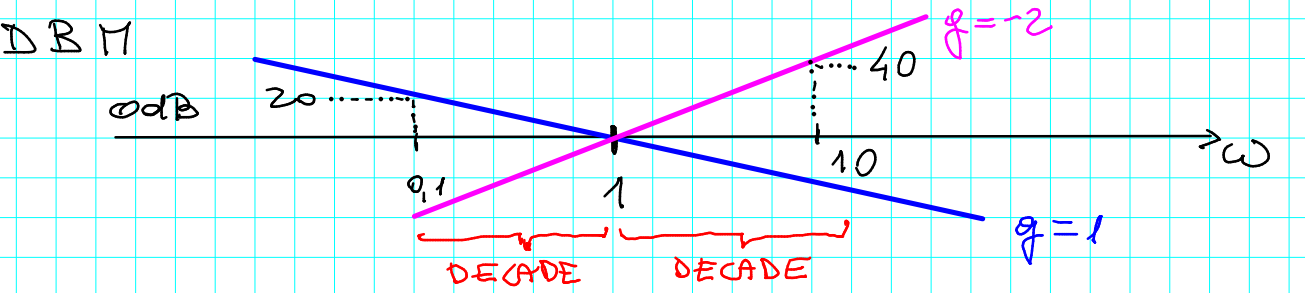
\includegraphics[height=3cm]{../lezione13/img1.PNG}
    \end{center}
    diagramma di bode del modulo: Il diagramma di bode del modulo corrispondente è una retta che interseca sempre l'asse delle ascisse nel punto $\omega = 1$ e la cui pendenza è $-20g \frac{dB}{decade}$ (spesso abbreviato come "pendenza $-g$"), dove la \textbf{decade} è la distanza corrispondente a un rapporto che vale $10$.\newline \newline
    diagramma di bode della fase: Il diagramma di bode delle fasi è orizzontale al valore $-g \cdot 90^o$. Anche per la fase spesso i termini $G_a$ e $G_b$ vengono analizzati assieme: il valore della retta orizzontale di $G_a$ e $G_b$ assieme è la semplice somma dei valori a cui dovrebbero essere le singole rette di $G_a$ e $G_b$\newline \newline
    Da notare è che fino ad ora non abbiamo fatto nessuna approssimazione.
    \item $G_c(s)= 1 + st \rightarrow  G_c(j \omega) = 1 + j \omega t \rightarrow \begin{cases}
        |G_c(j \omega)| = \sqrt{1 + (\omega t)^2}\\
        arg(G_c(j \omega))= arctan(\omega t)
    \end{cases}$\newline
    Per facilitare i conti applichiamo un approssimazione, che è il motivo del perchè stiamo facendo diagrammi di bode asintotici:
    \begin{itemize}
        \item se $| \omega t| >> 1$ (molto maggiore di $1$), allora $G_c(j \omega) \sim  j \omega t$, per cui otteniamo \newline che $\begin{cases}
            |G_c(j \omega)| \sim  | \omega t| \\
            arg(G_c(j \omega)) \sim  \begin{cases}
                90^o  \;\;& t>0\\
                -90^o & t <0
            \end{cases}
        \end{cases}$
        \item se $| \omega t| << 1$ (molto minore di $1$), allora $G_c(j \omega) \sim 1$, per cui otteniamo \newline ce $\begin{cases}
            |G_c(j \omega)| \sim  1 \\
            arg(G_c(j \omega)) \sim 0^o
        \end{cases}$
    \end{itemize}
    \ \newline
    [immagine dagli appunti del prof]
    \begin{center}
        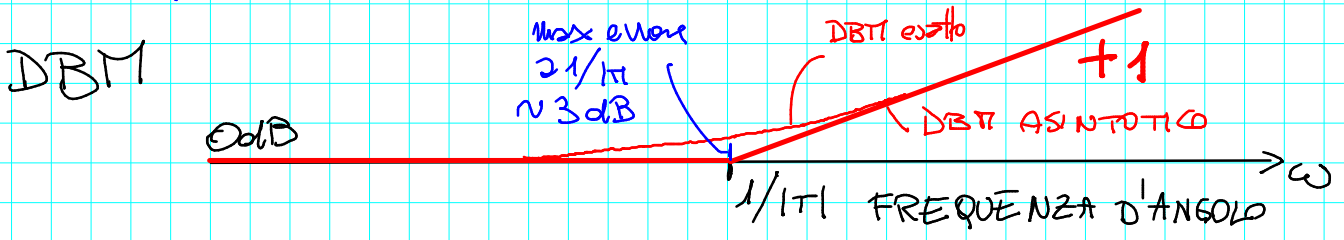
\includegraphics[height=2cm]{../lezione13/img2.PNG}
    \end{center}
    diagramma di bode del modulo: Definiamo la \textbf{frequenza d'angolo} come $\frac{1}{|t|}$ (da notare il modulo !). Grazie alle approssimazioni che abbiamo fatto, andando a sinistra nell'asse delle $\omega$, cioè verso il valore di $0 _{dB}$, il modulo vale circa $1$. Facciamo valere questa approssiamazione fino al valore di frequenza d'angolo. Superata la frequenza d'angolo il modulo cresce con pendenza $+1$, cioè di $20 \frac{dB}{decade}$. Questa rappresentazione prende il nome di diagramma di bode del modulo asintotico (il diagramma di bode del modulo esatto è mostrato in figura, e la differenza è che non ha una curva "netta").\newline \newline
    [immagine dagli appunti del prof]
    \begin{center}
        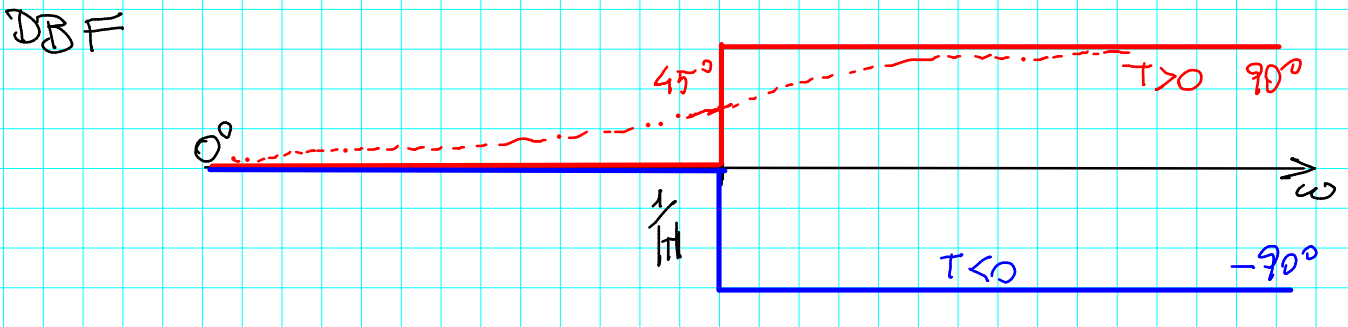
\includegraphics[height=3cm]{../lezione13/img3.PNG}
    \end{center}
    diagramma di bode della fase: approssimiamo tutto ciò che precede la frequenza d'angolo con $0^o$, alla frequenza d'angolo c'è un salto in cui se $t$ è positivo prota a $90^o$ (rossa nel disegno), se è negativo a $-90^o$ (blu nel disegno). La rappresentazione non approssimata dovrebbe seguire la linea tratteggiata in rosso nel disegno.\newline
    \newline
    Notiamo che l'approssimazione del modulo è molto buona, mentre quella della fase non molto.
    \item $G_d(s) = 1 + 2 \frac{\xi}{\omega_n}s + \frac{1}{\omega_n^2}s^2 \rightarrow  G_d(j \omega) = 1 + 2 \frac{\xi}{\omega_n} j \omega + \frac{1}{\omega_n^2}(j \omega)^2 = 1- \frac{\omega^2}{\omega_n^2} + j 2 \xi \frac{\omega}{\omega_n} $ con $1- \frac{\omega^2}{\omega_n^2}$ parte reale e $j 2 \xi \frac{\omega}{\omega_n}$ parte immaginaria
    \begin{itemize}
        \item per $\omega \rightarrow 0$: $\begin{cases}
            \text{parte reale}\; \rightarrow  1\\
            \text{parte immaginaria}\; \rightarrow 0
        \end{cases} \Rightarrow \begin{cases}
            |G_d(j \omega)| \rightarrow 1 \rightarrow |G_d(j \omega)|_{dB} \rightarrow 0\\
            arg(G_d(j \omega)) \rightarrow  0^o
        \end{cases}$ 
        \item per $\omega \rightarrow + \infty$: \newline
        [immagine dagli appunti del prof]
        \begin{center}
            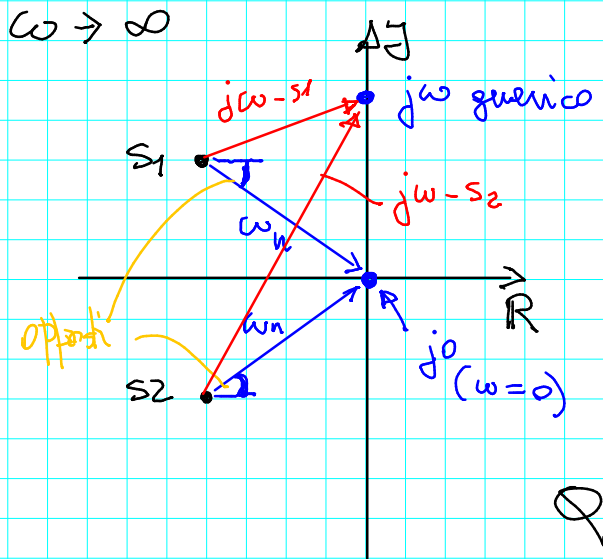
\includegraphics[height=6cm]{../lezione13/img4.PNG}
        \end{center}
        Chiamiamo le generiche radici coniugate complesse  la coppia $s_1$ e $s_2$ di $G_d(s) = \frac{1}{\omega_n^2}(s-s_1)(s-s_2)$ e rappresentiamole nel grafico.\newline \newline
        Facciamo un attimo un excursus dal caso $\omega \rightarrow  \infty$ e dimostriamo i risultati ottenuti precedentemente per $\omega \rightarrow 0$: [colore blu nel disegno] prendiamo il punto $j \omega$ con $\omega=0$, cioè $j0$, i vettori che connettono le radici $s_1$ e $s_2$ al punto $j0$ hanno modulo $\omega_n$, quindi il modulo di $|G_d(j0)|$ vale $\frac{\omega_n \cdot \omega_n}{\omega_n^2} = 1$. Possiamo anche dimostrare che la fase di $G_d$ per $\omega \rightarrow 0$, cioè in $j0$, che vale $0^o$, infatti gli angoli di $s_1$ e $s_2$ rispetto a un asse orizzontale sono opposti e si annullano a vicenda.\newline \newline
        Vediamo ora il caso in cui, invece di considerare il punto $j0$, consideriamo il generico punto $j \omega$. Analiziamo i vettori che connettono il generico punto $j \omega$ e $s_1$ e $s_2$ [in rosso nel disegno], questi vettori $j \omega - s_i$ per $\omega \rightarrow \infty$ (cioè per facendo salire lungo l'asse immaginario il generico punto $j \omega$) hanno entrami modulo che tende a $\infty$ e fase che tende a $90^o$ (quindi in totale $180^o$).\newline
        Quindi per $\omega \rightarrow  \infty \Rightarrow \begin{cases}
            |G_d(j \omega)| \rightarrow \infty \;\;\text{allo stesso modo in cui tende}\;\omega^2\\
            arg(G_d(j \omega)) \rightarrow  180^o
        \end{cases}$ \newline
        \newline
        [immagine dagli appunti del prof]
        \begin{center}
            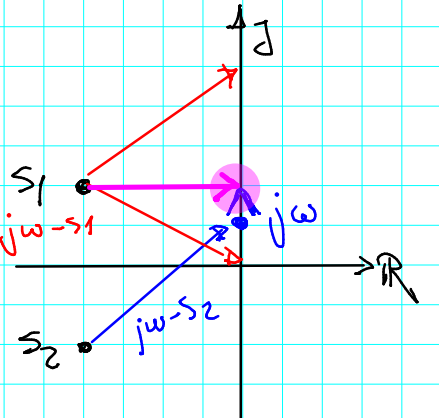
\includegraphics[height=6cm]{../lezione13/img5.PNG}
        \end{center}
        \textbf{oss.} Il modulo del vettore $|j \omega - s_2|$ è monotono crescente, mentre il modulo del vettore $|j \omega - s_1|$ no, infatti ha un minimo per $\omega = Im(s_1)$, il perchè si vede graficamente.\newline
        \newline
        \textbf{oss.} più $s_1$ e $s_2$ sono vicini all'asse immaginario, più il minimo di $s_1$ è pronunciato e la variazione di fase avviene bruscamente.\newline
        \newline
        [immagine dagli appunti del prof]
        \begin{center}
            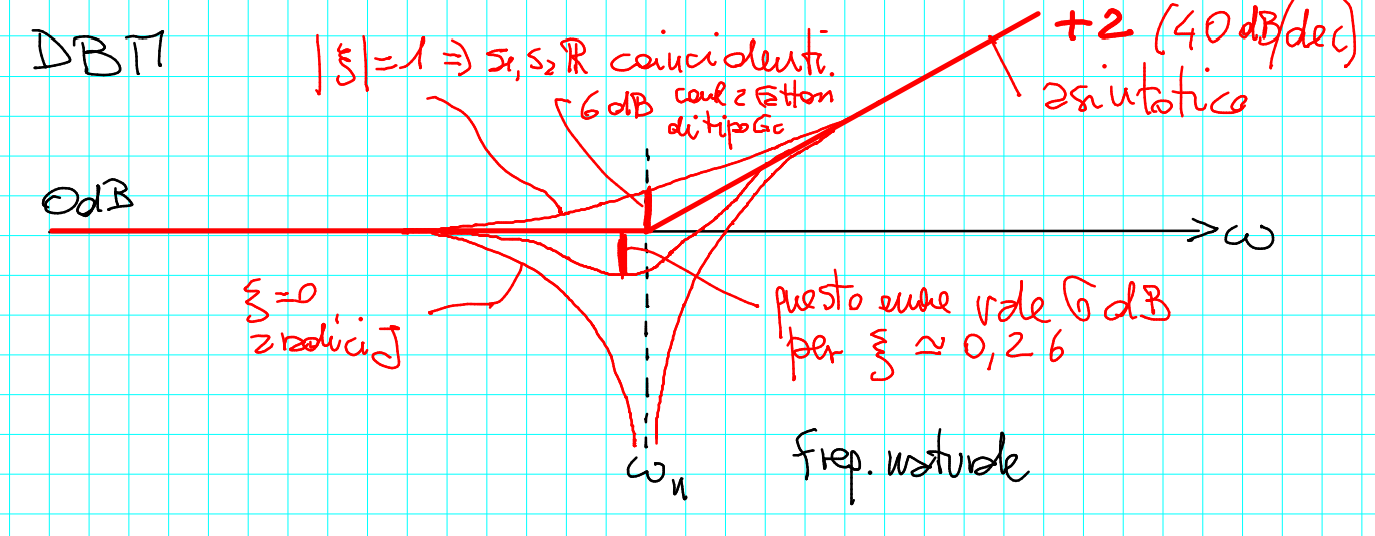
\includegraphics[height=4cm]{../lezione13/img6.PNG}
        \end{center}
        Diagramma di Bode del modulo: Segnamo la frequenza $\omega_n$ che prende il nome di \textbf{frequenza naturale}. Approssimiamo tutto ciò che precede $\omega_n$ con modulo uguale a $1$ ($0dB$), invece dalla frequenza naturale in poi il modulo sale con pendenza $+2$ (cioè $40 \frac{dB}{decade}$). Questo è il diagramma asintotico. Il diagramma esatto è mostrato in figura ed è diverso in base al termine $\xi$ ($|\xi| = 1$ abbiamo due radici reali coincidenti, $|\xi| = 0$ abbiamo $2$ radici immaginarie, in mezzo a questi due casi ci sono tutti gli altri casi possibili)\newline
        \newline
        [immagine dagli appunti del prof]
        \begin{center}
            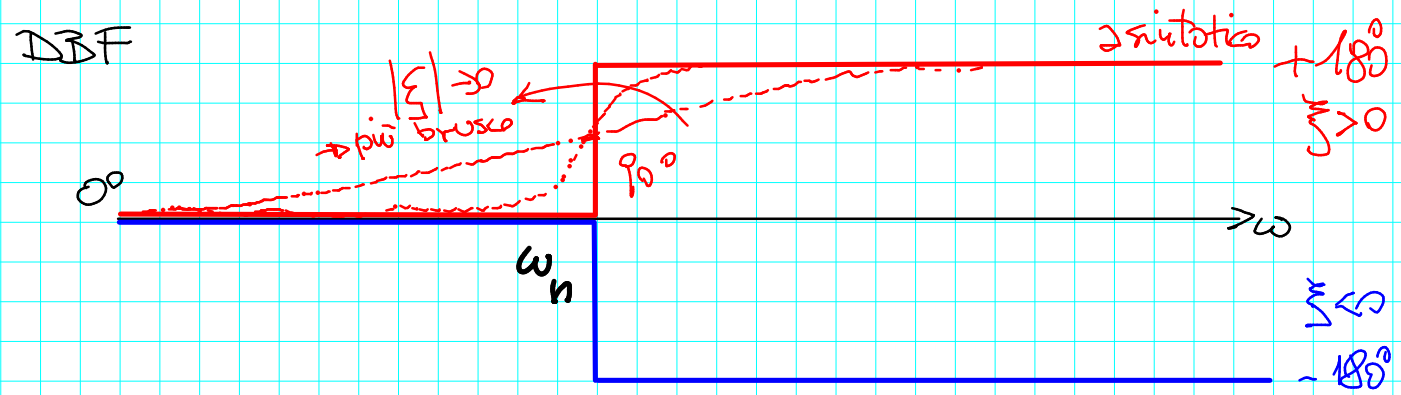
\includegraphics[height=3cm]{../lezione13/img7.PNG}
        \end{center}
        Diagramma di Bode della fase: Il diagramma asintotico (approssimato) è fatto a scalino e va da $0^o$ a $+ 180^o$ se $\xi > 0$ o a $-180^o$ se $\xi < 0$. Il diagramma esatto è mostrato in figura (tratteggiato in rosso) e può avere una pendenza più o meno ripida per $|\xi| \rightarrow 0$.
    \end{itemize} 
\end{itemize}
\subsubsection{Tracciamento complessivo}
Per capire come unire tutti i diagrammi fino ad ora visti di $G_{a,b,c,d}$ vediamo un esempio. \newline
\newline
\textbf{es.} Sia $G(s) = \frac{10(1-s)(1+\frac{s}{2})}{s(1+ \frac{s}{10})^2}$, con $\mu=10$ e $g=1$. Riscriviamolo per una migliore comprensione come:
\[
    G(s) = \frac{10}{s} \cdot  (1-s) \cdot  (1+\frac{s}{2}) \cdot \frac{1}{1 + \frac{s}{10}} \cdot  \frac{1}{1+\frac{s}{10}}
\]
\ \newline
Facciamo ora i diagrammi di bode del modulo di tutti questi termini e infine li sommiamo per avere il diagramma complessivo.\newline
\newline
[immagine dagli appunti del prof]
\begin{center}
    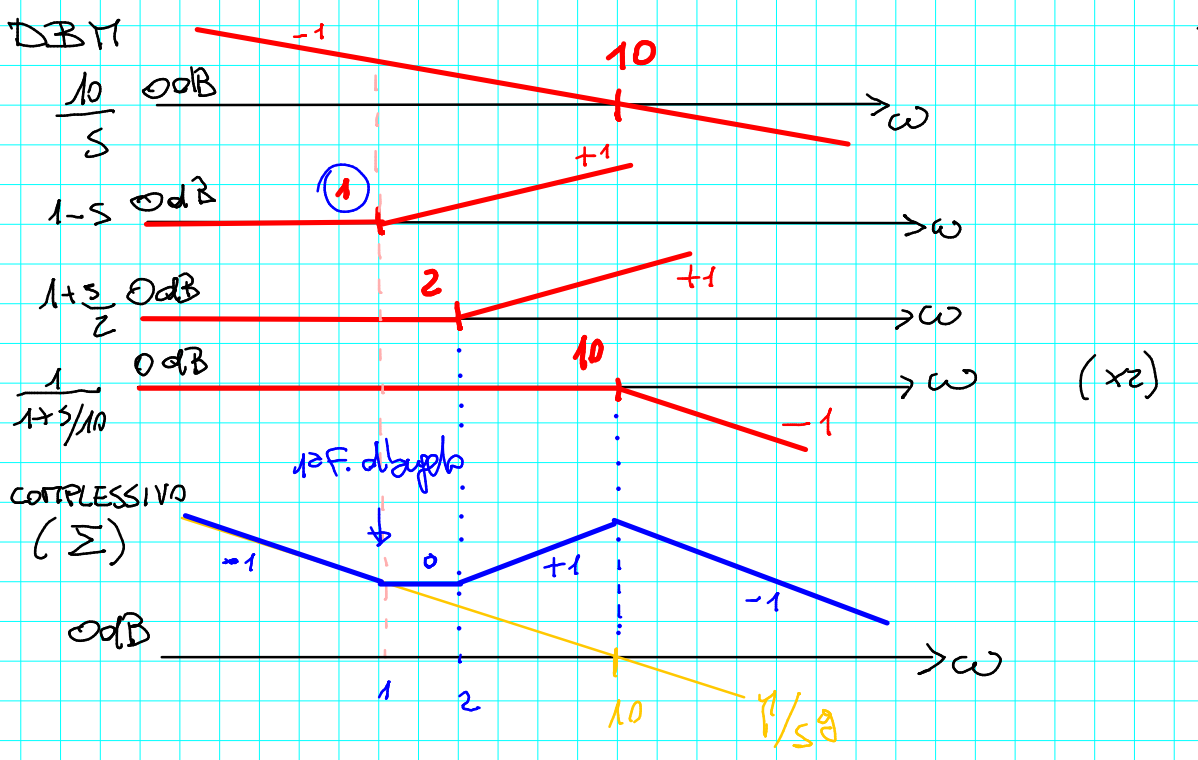
\includegraphics[height=7cm]{../lezione13/img8.PNG}
\end{center}
\begin{itemize}
    \item $\frac{10}{s}$: pendenza $-1$ e intersezione con l'asse $\omega$ in $10$.
    \item $(1-s)$: parte da $0$ e alla frequenza d'angolo $1$ ottiene pendenza $+1$. 
    \item $(1+\frac{s}{2})$: vale $0$ fino a frequenza $2$ e poi sale con pendenza $+1$. 
    \item $\frac{1}{1 + \frac{s}{10}}$ (di cui ce ne sono due identici, da ricordare per fare il diagramma complessivo finale): vale $0$ fino a frequenza d'angolo $10$ e poi ottiene pendenza (scende) $-1$, perchè essendo a denominatore il logaritmo cambia segno.
    \item diagramma di bode complessivo: è la somma dei diagrammi precedenti, graficamente si può ragionare sul fatto che il diagramma complessivo è fatto da dei semplici cambi di pendenza dovuti a tutti i diagrammi precedenti. (notiamo che l'ultimo termine è presente due volte).
\end{itemize}
\ \newline
\newline
Facciamo ora i diagrammi di bode della fase di tutti questi termini e infine li sommiamo per avere il diagramma complessivo.\newline
\newline
[immagine dagli appunti del prof]
\begin{center}
    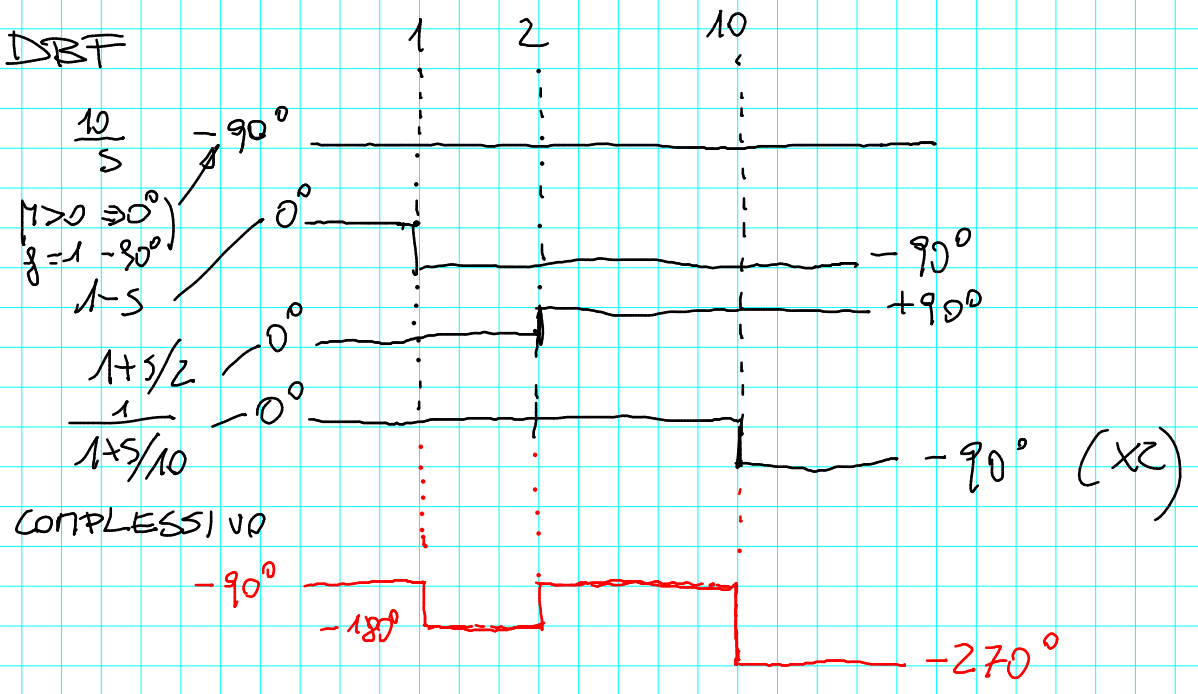
\includegraphics[height=7cm]{../lezione13/img9.PNG}
\end{center}
\begin{itemize}
    \item $\frac{10}{s}$: è una retta orizzontale a $-90^o$ fissi.
    \item $(1-s)$: parte da $0^o$ e poi ha uno scalino negativo fino a $-90^o$ (negativo perchè è del tipo $1-j \omega$) alla frequenza di $\omega=1$.
    \item $(1+\frac{s}{2})$:  parte da $0^o$ e alla sua frequenza d'angolo che vale $2$ ha uno scalino in cui passa a $+ 90^o$ (positivo perchè è del tipo $1+j \omega$).
    \item $\frac{1}{1 + \frac{s}{10}}$ (di cui ce ne sono due identici, da ricordare per fare il diagramma complessivo finale): parte da $0^o$ e alla frequenza di $10$ ha uno scalino fino a $-90^o$ (è della forma $1 + j \omega$, ma \textbf{siccome è al denominatore il segno viene cambiato}, quindi è negativo)
    \item diagramma di bode complessivo: è la somma dei diagrammi precedenti, graficamente si può ragionare sul fatto che il diagramma complessivo è fatto dalla somma dei vari scalini alla frequenza opportuna. (notiamo che l'ultimo termine è presente due volte).
\end{itemize}
\ \newline
\newline
\textbf{In generale per la fase}: Se è del tipo $1+j \omega$ allora abbiamo uno scalino positivo di $+90^o$ gradi alla frequenza d'angolo, se è del tipo $1- j \omega$ allora abbiamo uno scalino negativo di $-90^o$ alla frequenza d'angolo. Se invece il termine $1\pm j \omega$ è a denominatore, il ragionamento è al contrario, cioè se è del tipo $\frac{1}{1+j \omega}$ allora abbiamo uno scalino negativo di $-90^o$ alla frequenza d'angolo, se è del tipo $\frac{1}{1- j \omega}$ allora abbiamo uno scalino positivo di $+90^o$ alla frequenza d'angolo.
\subsubsection{Metodo di tracciamento}
Per prima cosa si ricavano i valori di $\mu$, $g$, poi si ricavano tutte le frequenze d'angolo (modulo delle radici di ogni termine al numeratore e al denominatore, escluse quelle in $s=0$) e per ognuna di queste si dice quanti zeri (radici del numeratore) destri (con parte reale positiva) o sinistri (con parte reale negativa) e quanti poli (radici del denominatore) destri (con parte reale positiva) o sinistri (con parte reale negativa) ci sono.\newline
\newline
\textbf{Diagramma di Bode del modulo}: 
\begin{enumerate}
    \item Tracciare il diagramma di Bode del modulo di $\frac{\mu}{s^g}$ (è una retta la cui pendenza viene ricavata da: $-20 \cdot g \frac{dB}{decade}$; per capire dove interseca l'asse delle $\omega$ basta ricavare il valore di $\omega$ per cui $\left| \frac{\mu}{\omega^g} \right| = 1$; se la retta non ha pendenza allora è una retta orizzontale all'altezza di $|\mu|_{dB}$).
    \item Segnare sull'asse delle $\omega$ le frequenze d'angolo dei poli (radici del denominatore) e zeri (radici del numeratore) non in $s=0$ (perchè son già presenti nel punto precedente).\newline
    Quando si incontra una frequenza d'angolo di uno zero, la pendenza aumenta di $1$, quando si incontra una frequenza d'angolo di un polo, la pendenza diminuisce di $1$. (Ricordiamo che per 1 di pendenza si intendono $20 dB/decade$).
\end{enumerate}
\textbf{Diagramma di Bode della fase}:
\begin{enumerate}
    \item Il diagramma di Bode della fase parte al valore di $arg(\frac{\mu}{(j \omega)^g})$, che è calcolabile sommando i contributi di $\mu$ e $\frac{1}{s^g}$ nel seguente modo:
    \[
        \mu \rightarrow \begin{cases}
            0^o \;\;\;& se > 0\\
            -180^o \;\;\; & se <0
        \end{cases} \;\;\;\;\;\;\;\;\;\;\;\;\;\;\; \frac{1}{s^g}\rightarrow -g \cdot 90^o
    \]
    \item zero "a sinistra" la fase aumenta di $90^o$;\newline
    zero "a destra" la fase diminuisce di $90^o$;\newline
    polo "a sinistra" la fase diminuisce di $90^o$;\newline
    polo "a destra" la fase aumenta di $90^o$.
\end{enumerate}
\subsubsection{Esempio}
\textbf{es.} Disegnare i diagrammi di Bode asintotici per la funzione di trasferimento 
\[
    G(s) = \frac{100(1-s)(1+ \frac{s}{5})}{s^2(1-\frac{s}{10})(1+ \frac{s}{100})^2}
\]
$\mu = 100$ e $g=2 \; \Rightarrow  \; \frac{\mu}{s^g}$ ha pendenza $-2$ e taglia l'asse delle $\omega$ per $\frac{100}{\omega^2} =1$ cioè per $\omega =10$.\newline
\newline
Frequenze d'angolo di poli e zeri non nell'origine:
\[
    \begin{matrix}
        \omega = 1 \;\;\;\;\; & 1 \;\text{zero destro}\; \\
        \omega = 5 \;\;\;\;\; & 1 \;\text{zero sinistro}\; \\
        \omega = 10 \;\;\;\;\; & 1 \;\text{polo destro}\; \\
        \omega = 100 \;\;\;\;\; & 2 \;\text{poli sinistri }\; \\
    \end{matrix}
\]
Usiamo ora il foglio semilogaritmico (che si può trovare fra i materiali del corso sul sito del professore):\newline
\newline
[immagine dagli appunti del prof]
\begin{center}
    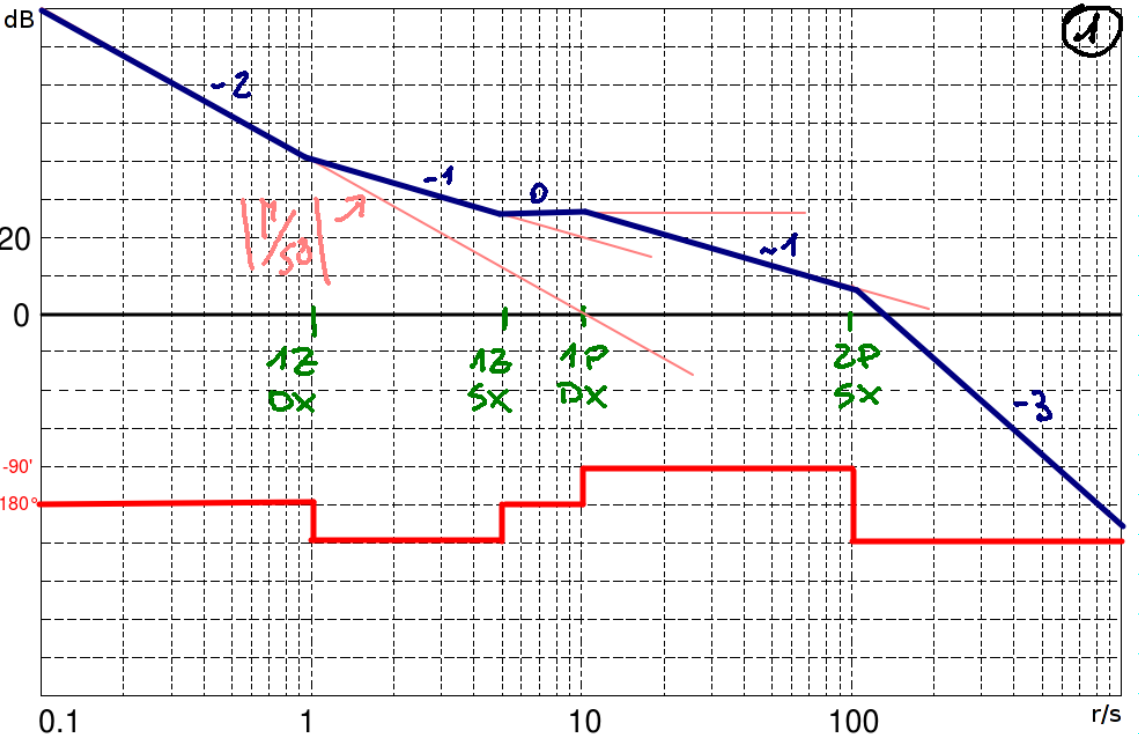
\includegraphics[height=7cm]{../lezione13/img10.PNG}
\end{center}
Notiamo che per convenzione si rappresentano $10dB$ a tacca (verticale), inoltre se mancano le scale nel diagramme di bode si considera errore in sede d'esame!
\rule{\textwidth}{0,4pt}